\documentclass[border=10pt]{standalone}

\usepackage{tikz}
\usepackage{tikzsymbols}
\usetikzlibrary{calc,patterns,shapes.geometric}

\def\centerarc[#1](#2)(#3:#4:#5){\draw[#1] ($(#2)+({#5*cos(#3)},{#5*sin(#3)})$) arc (#3:#4:#5);}

\begin{document}
	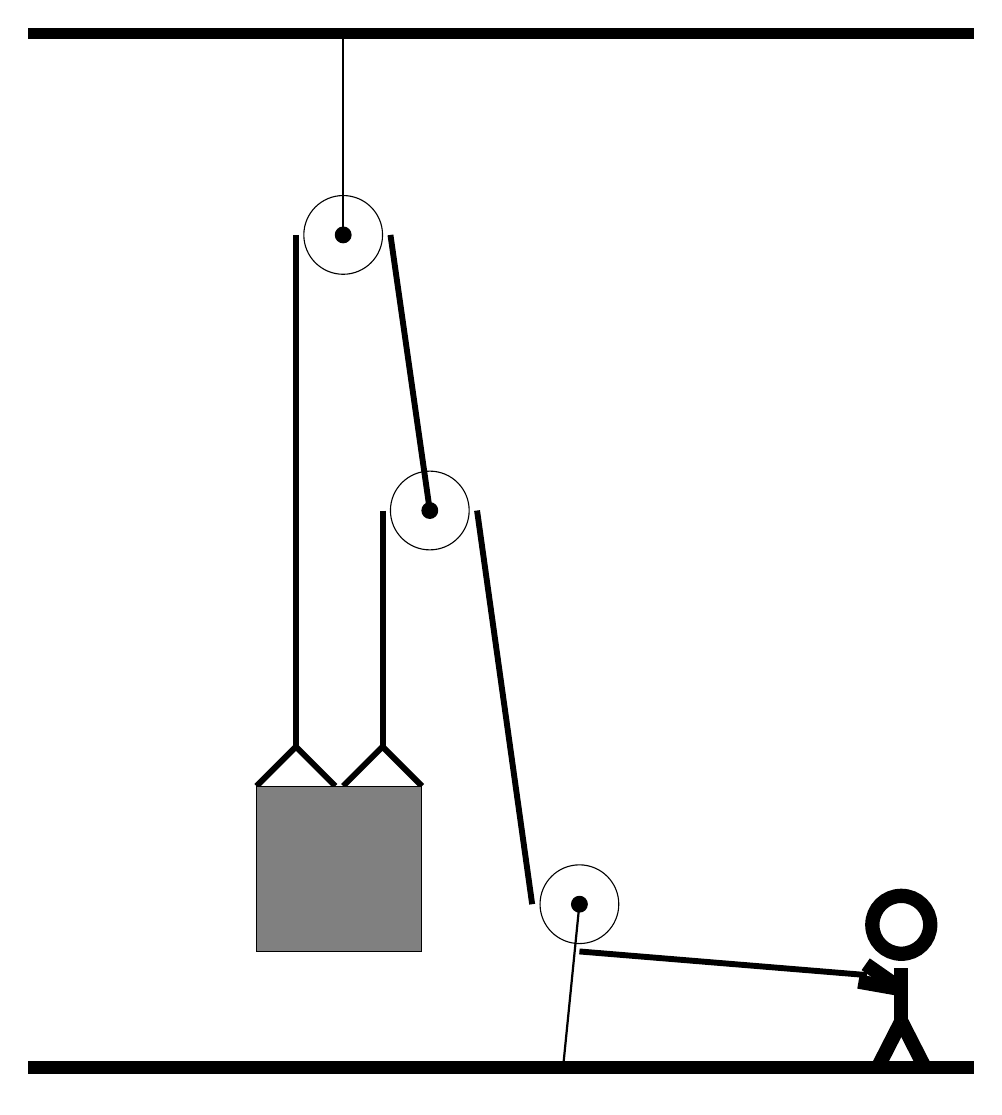
\begin{tikzpicture}
		%%%%% START %%%%%
		\draw[fill=black] (-2, 10) rectangle (10, 10.125);
		
		\draw (2, 7.5) circle (0.5);
		\draw[fill=black] (2, 7.5) circle (0.1);
		\draw[thick] (2, 7.5) -- (2, 10);
		
		\draw (3.1, 4.0) circle (0.5);
		\draw[fill=black] (3.1, 4.0) circle (0.1);
		
		\draw (5, -1) circle (0.5);
		\draw[fill=black] (5, -1) circle (0.1);
		\draw[thick] (5, -1) -- (4.8, -3);
		
		\draw[line width = 0.75mm]  (0.9, 0.5) -- (1.4, 1.0) -- (1.9, 0.5);
		\draw[line width = 0.75mm]  (2.0, 0.5) -- (2.5, 1.0) -- (3.0, 0.5);
		\draw[fill=black!50] (0.9, 0.5) rectangle (3.0, -1.6);
		
		\draw[line width = 0.75mm] (1.4, 7.5) -- (1.4, 1.0);
		\centerarc[line width = 0.75mm](2, 7.5)(0:180:0.6);
		\draw[line width = 0.75mm] (2.6, 7.5) -- (3.1, 4.0);
		\draw[line width = 0.75mm] (2.5, 4.0) -- (2.5, 1.0);
		\centerarc[line width = 0.75mm](3.1, 4.0)(0:180:0.6);
		\draw[line width = 0.75mm] (3.7, 4.0) -- (4.4, -1);
		\centerarc[line width = 0.75mm](5, -1)(180:270:0.6);
		\draw[line width = 0.75mm] (5, -1.6) -- (8.65, -1.9);
		
		\node at (9, -2) {\Strichmaxerl[10][-35][170]};
		
		\draw[fill=black] (-2, -3) rectangle (10, -3.15);
		%%%%% END %%%%%
	\end{tikzpicture}
\end{document}